%
%
%% Section: DEPLOYMENT
%\section{Community Cloud Deployment}
%\label{sec:deployment}
%
%\begin{figure}[tbp]
%   \centering
%   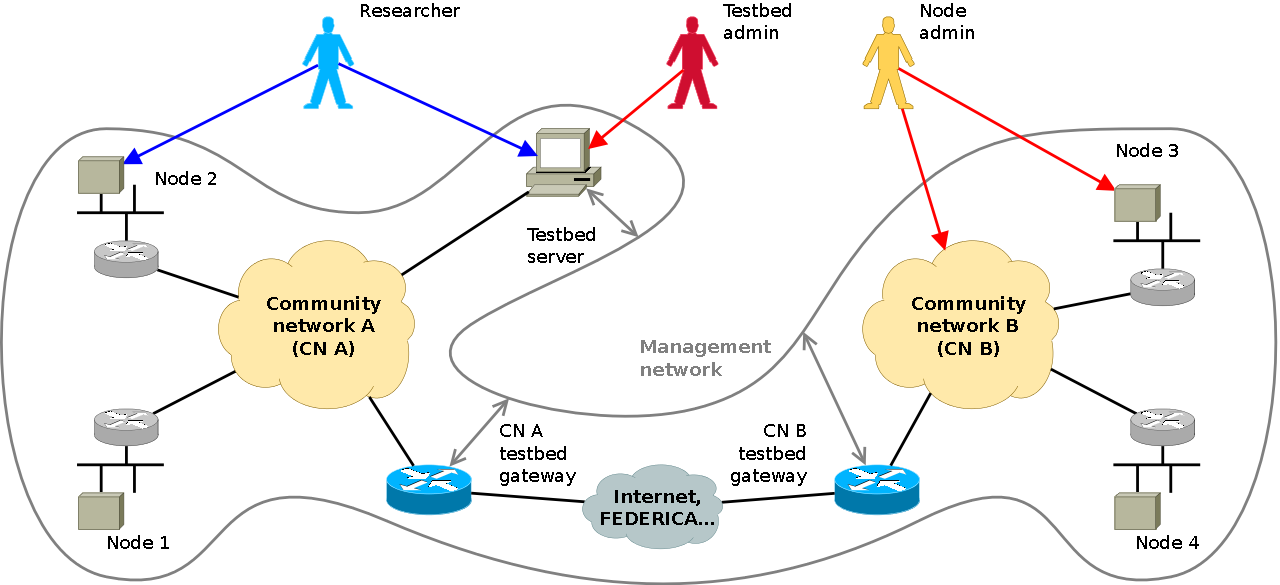
\includegraphics[width=3.1in,keepaspectratio]{confine_testbed_arch}
%   \caption{Experiment setup using Community-Lab testbed, with Guifi.net and AWMN connected through FEDERICA}
%   \label{fig:confine_testbed_arch}
%\end{figure}
%
%We explain in this section our current work in setting up a prototype cloud infrastructure 
%in Guifi.net and Athens Wireless Metropolitan Network (AWMN)\footnote{\url{http://www.awmn.net}} community networks, 
%and present results from our experiments with distributed storage and data sharing service running in this testbed.
%
%%%%%%%%%%%%%%%%%%%%%%%%%%%%%%%%%%%%%%%
%\subsection{Experiment Environment: Community-Lab Testbed}
%
%For having a realistic community network setting for the collaborative cloud services, 
%we have used Community-Lab\footnote{\url{http://community-lab.net}} testbed for setting up our community cloud infrastructure.
%Community-Lab is a distributed infrastructure developed by the CONFINE project~\cite{Braem2013}, 
%where researchers can deploy experimental services on several nodes deployed within federated community networks. 
%Community-Lab provides IaaS for community clouds by providing the researchers with a set of VMs, implemented as Linux containers (LXC), from the nodes which are distributed within the community network. 
%Within these VMs we deploy Cloudy\footnote{\url{http://repo.clommunity-project.eu}}~\cite{Jimenez2014},
%a Debian based distribution, 
%which comes pre-installed with some of the collaborative distributed applications, 
%like Tahoe-LAFS\footnote{\url{https://tahoe-lafs.org}}, ownCloud, etc.
%
%The primary configuration for our application deployments consists of nodes from the two community networks, Guifi.net in Spain and AWMN in Greece, which are connected on the IP layer though Federated E-infrastructure Dedicated to European Researchers (FEDERICA)\footnote{\url{http://www.fp7-federica.eu}}, enabling network federation, as illustrated in Figure~\ref{fig:confine_testbed_arch}. 
%This implies that some part of the distributed applications are in fact spread over nodes in Guifi.net, while the other components are hosted on the nodes belonging to AMWN. 
%The nodes of our experiments are the real nodes from both the community networks, and they are connected to other actively used nodes within the community network through wireless IEEE 802.11 a/b/n connections.
%
%
%%%%%%%%%%%%%%%%%%%%%%%%%%%%%%%%%%%%%%%
%\subsection{Collaborative Cloud Services}
%
%We present here a brief overview of the different collaborative cloud services that we are exploring and planning to deploy in our community cloud testbed based on Community-Lab.
%
%\subsubsection[IaaS]{Infrastructure-as-a-Service (IaaS)}
%We have set up different machines with 
%	OpenStack, 
%	Eucalyptus, 
%	Proxmox\footnote{\url{http://proxmox.com/}}, 
%	Docker.io\footnote{\url{http://docker.com}} 
%	and OpenWRT/LXC installations, 
%which provide either a virtual machine or Linux container based environment. 
%All the nodes share the same Guifi.net IP-address space and are network reachable.
%This means that they can support applications and services deployed on the federated infrastructure from multiple cloud setups. 
%
%\subsubsection[PaaS]{Platform-as-a-Service (PaaS)}
%We set up a storage service (based on Tahoe-LAFS and ownCloud) and a database service (based on CATS project's Caracal database\footnote{\url{http://cats.sics.se}}) at platform level to support the development of cloud applications for the end users. 
%The Debian-based Cloudy distribution\cite{Jimenez2014} also integrates support services, like Avahi\footnote{\url{http://avahi.org}} which provides services discovery and management.
%
%\subsubsection[SaaS]{Software-as-a-Service (SaaS)}
%We are also looking into providing useful collaborative services for the end users because these application are critical for the uptake of community cloud model among the existing users of community networks.
%For instance, we are setting up collaborative distributed storage service 
%using a combination of ownCloud, XtreemFS\footnote{\url{http://xtreemfs.org}} and Tahoe-LAFS, 
%and video streaming service using PeerStreamer~\cite{Birke2012} and PeerTV~\cite{Payberah2010}. 
%
